\documentclass[conference,compsoc]{IEEEtran}
\newcommand\tab[1][0.75cm]{\hspace*{#1}}
\usepackage[utf8]{inputenc}

\ifCLASSOPTIONcompsoc
   \usepackage[nocompress]{cite}
\else
 
  \usepackage{cite}
\fi


\usepackage[pdftex]{hyperref}


% *** GRAPHICS RELATED PACKAGES ***

\ifCLASSINFOpdf
   \usepackage{graphicx}
   \graphicspath{{files/}}
  
\else
 
\fi
% correct bad hyphenation here
\hyphenation{op-tical net-works semi-conduc-tor}

%********** Começo do documento ************88

\begin{document}



\title{Ponto de controle 3\\Fechadura digital para controle e monitoramento para unidades de terapia intensiva}



\author{
\IEEEauthorblockN{João Vitor Rodrigues Baptista}
\IEEEauthorblockA{15/0013329\\UnB - FGA \\
Brasília, Brasil \\
Email: jvrbaptista@live.com }
\and
\IEEEauthorblockN{Igor Sousa Nunes de Oliveira}
\IEEEauthorblockA{15/0011971\\
UnB - FGA \\
Brasília, Brasil\\
Email: igorsno97@gmail.com }}

\maketitle

% As a general rule, do not put math, special symbols or citations
% in the abstract
\begin{abstract}
Colocar um abstrat aqui...
As a general rule, do not put math, special symbols or citations
in the abstract
\end{abstract}

\IEEEpeerreviewmaketitle



\section{Introdução}

O controle de acessos ou mesmo a restrição de pessoas a algum ambiente é algo muito comum no cotidiano e que de forma mais comum são utilizadas catracas, portas giratórias entre outras maneiras para o controle do ambiente ou mesmo como permissão para entrada ou saída de pessoas em um ambiente controlado.

Partindo dessa situação é proposto neste relatório a criação de uma fechadura de liberação de acessos digital para o controle do ambiente com uma aplicação em um sistema aplicado em uma unidade de terapia intensiva.

\begin{figure}[!ht]
		\centering
		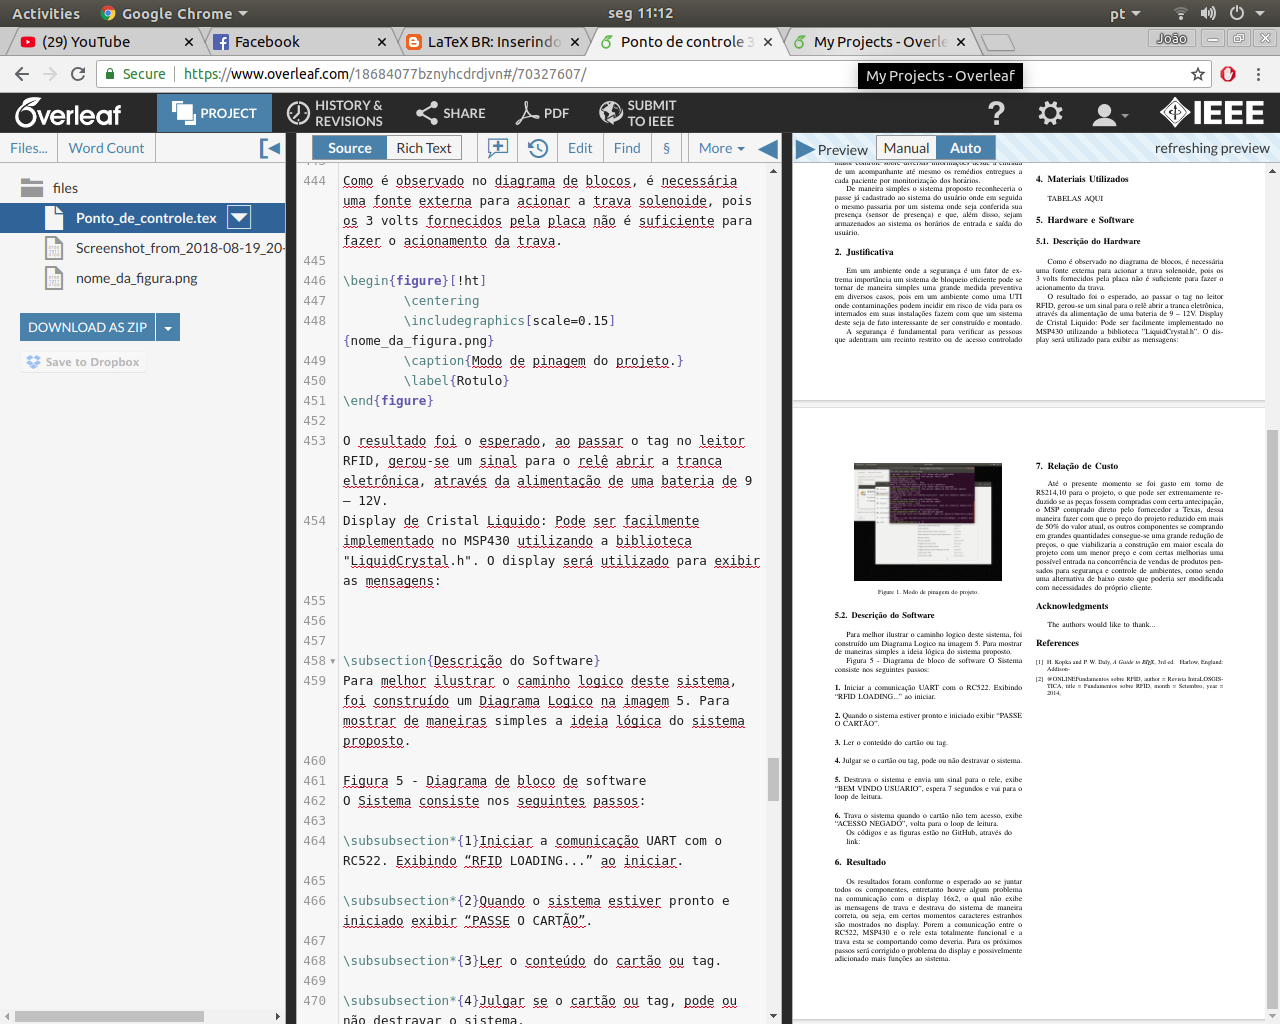
\includegraphics[scale=0.15]{nome_da_figura2.png}
		\caption{Figura 2}
		%\label{Rotulo}
\end{figure}

Usando por meio de identificadores de rádio frequência (RFID), pode-se ser montado um meio de controle que dá mesma maneira que possa se manter um ambiente seguro, possa de maneira prática manter a transição de pessoas em ambientes controlados, a fim de se manter em controle infecções, doenças entre diversos outros além de ter um maior controle sobre diversas informações desde a entrada de um acompanhante até mesmo os remédios entregues a cada paciente por monitorização dos horários.

De maneira simples o sistema proposto reconheceria o passe já cadastrado ao sistema do usuário onde em seguida o mesmo passaria por um sistema onde seja conferida sua presença (sensor de presença) e que, além disso, sejam armazenados ao sistema os horários de entrada e saída do usuário.


\section{Justificativa}
Em um ambiente onde a segurança é um fator de extrema importância um sistema de bloqueio eficiente pode se tornar de maneira simples uma grande medida preventiva em diversos casos, pois em um ambiente como uma UTI onde contaminações podem incidir em risco de vida para os internados em suas instalações fazem com que um sistema deste seja de fato interessante de ser construído e montado.

A segurança é fundamental para verificar as pessoas que adentram um recinto restrito ou de acesso controlado e pessoas desconhecidas que podem tentar entrar no lugar, por isso deve ser feito o monitoramento de horários de quem entra e sai do local, evitando-se possíveis invasões , o que pode ser bastante perigoso em diversos casos, onde se tem diversas doenças infectocontagiosas, pacientes com grande risco.

 Portanto em um ponto de vista prático sobre o projeto se torna interessante por poder defender a integridade dos pacientes que estão normalmente sobre situações mais complicadas e dessa maneira poder ter um acréscimo na qualidade apresentada em tais unidades.
 
 \section{Objetivos}
Identificar as pessoas que entram e saem além de poder ter controle dos tempos de acessos de cada pessoa individualmente e armazenar em um banco de dados. Barrar a entrada de elementos indesejáveis no recinto de maneira prática, tornando o ambiente mais seguro e propício à melhora dos pacientes e de riscos minimizados.
%---------------------  ----------------------

\section{Materiais Utilizados}
TABELAS AQUI

\begin{table}[tbp]
\caption{Tabela 1 - Exemplo}
\label{my-label}
\begin{tabular}{ccccc}
\textbf{Nome}   & \textbf{Nome1} & \textbf{Nome2} & \textbf{Nome3} & \textbf{Nome4} \\
\textbf{Nome11} & 1              & 2              & 3              & 4              \\
\textbf{Nome21} & 5              & 6              & 7              & 8              \\
\textbf{Nome31} & 9              & 10             & 11             & 12            
\end{tabular}
\end{table}
%---------------------  ----------------------

\section{Hardware e Software}

%---------------------  ----------------------
\subsection{Descrição do Hardware}

Como é observado no diagrama de blocos, é necessária uma fonte externa para acionar a trava solenoide, pois os 3 volts fornecidos pela placa não é suficiente para fazer o acionamento da trava.

\begin{figure}[!ht]
		\centering
		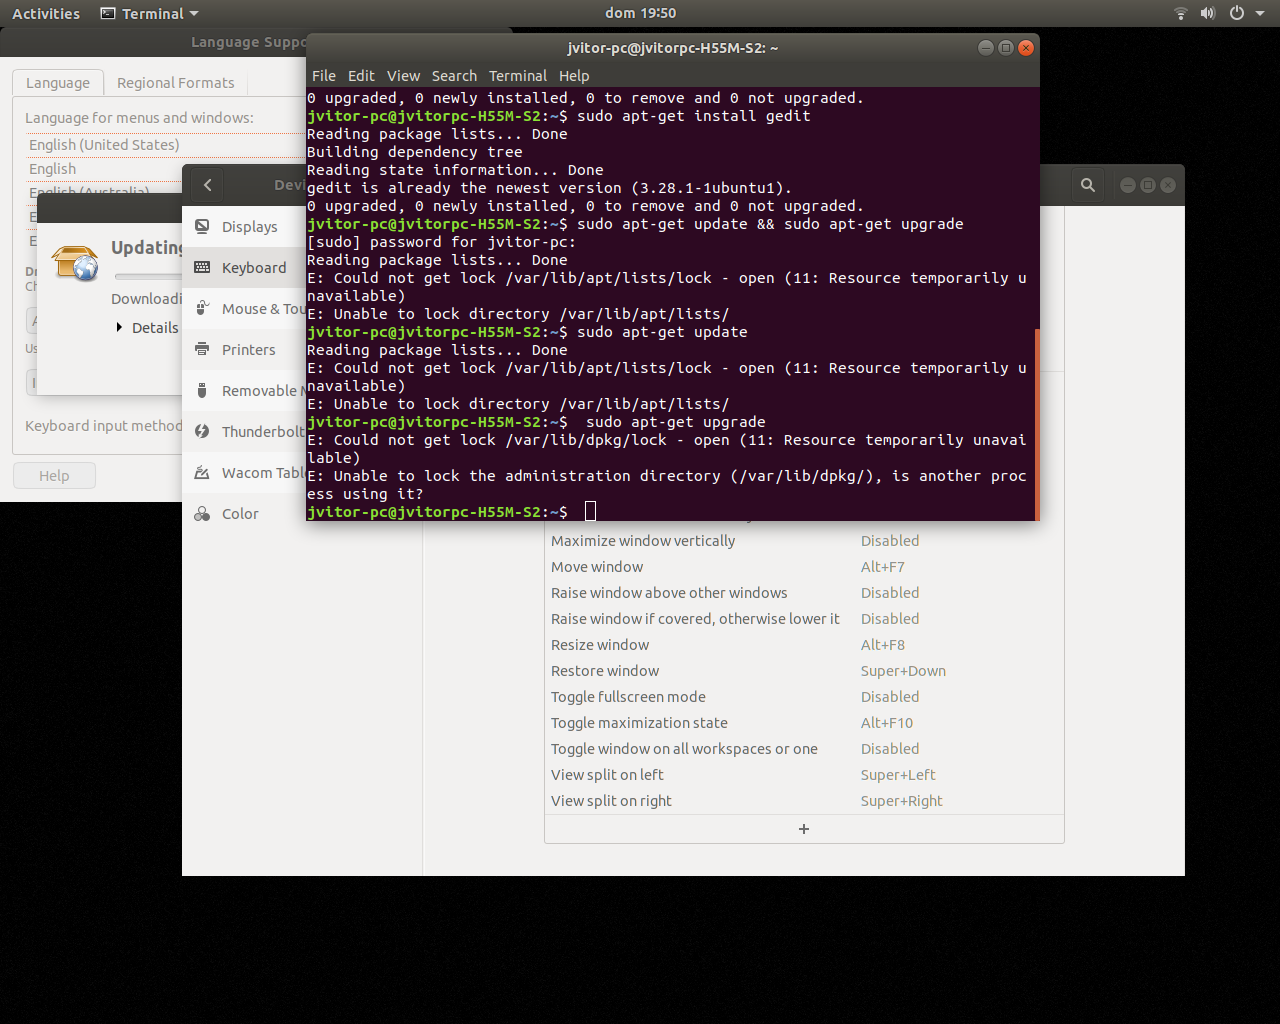
\includegraphics[scale=0.15]{nome_da_figura.png}
		\caption{Figura 1.}
		%\label{Rotulo}
\end{figure}

O resultado foi o esperado, ao passar o tag no leitor RFID, gerou-se um sinal para o relê abrir a tranca eletrônica, através da alimentação de uma bateria de 9 – 12V. 
Display de Cristal Liquido: Pode ser facilmente implementado no MSP430 utilizando a biblioteca "LiquidCrystal.h". O display será utilizado para exibir as mensagens:

%---------------------  ----------------------


\subsection{Descrição do Software}
Para melhor ilustrar o caminho logico deste sistema, foi construído um Diagrama Logico na imagem 5. Para mostrar de maneiras simples a ideia lógica do sistema proposto.
 \begin{figure}[!ht]
		\centering
		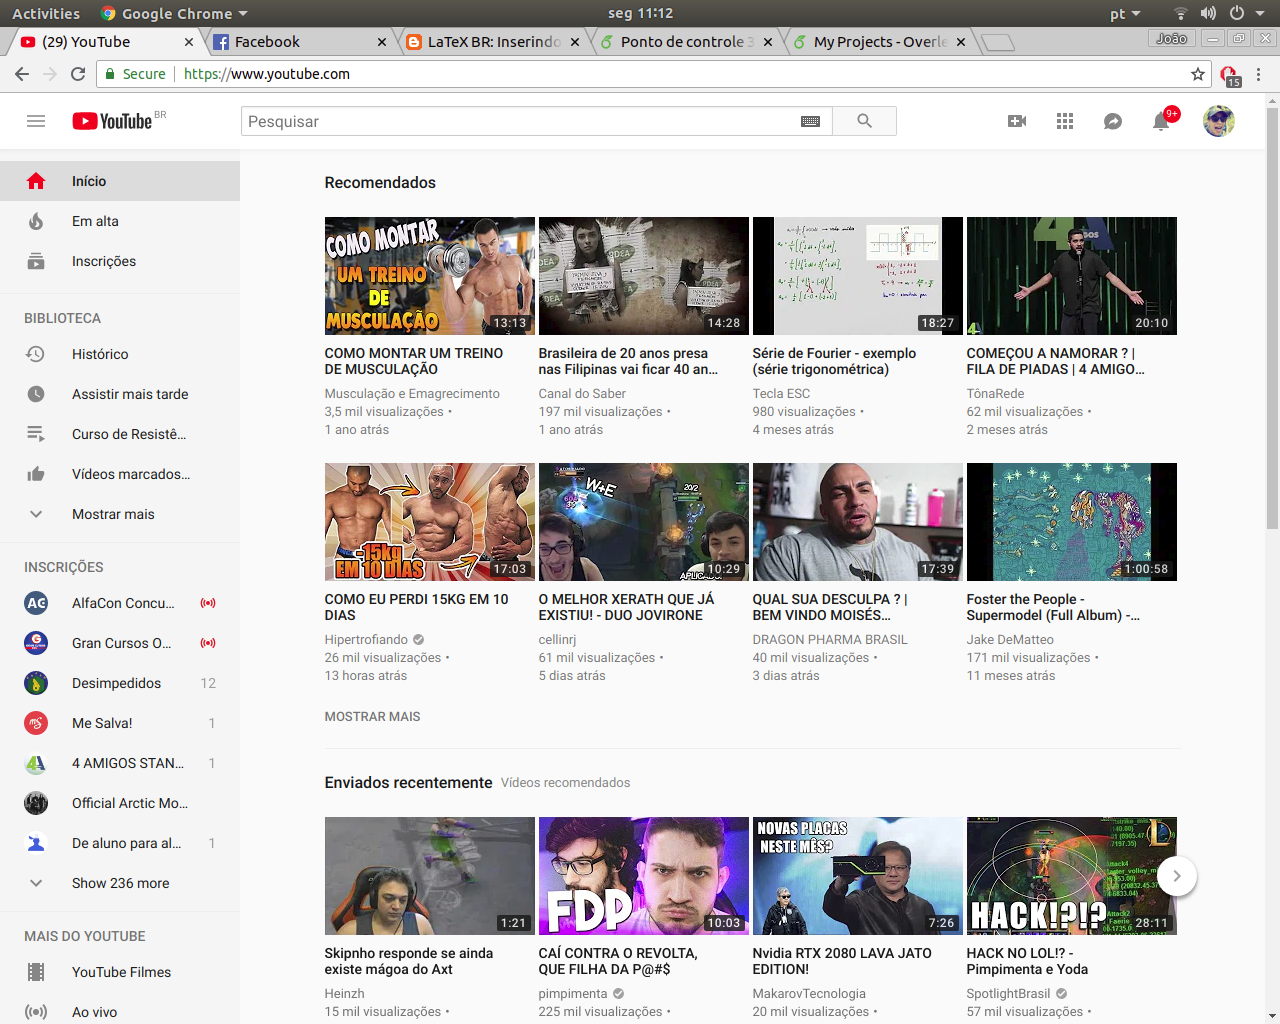
\includegraphics[scale=0.15]{nome_da_figura1.png}
		\caption{Figura 1}
		%\label{Rotulo}
\end{figure}

O Sistema consiste nos seguintes passos:

\tab 1. Iniciar a comunicação UART com o RC522. Exibindo “RFID LOADING...” ao iniciar.

\tab 2. Quando o sistema estiver pronto e iniciado exibir “PASSE O CARTÃO”.

\tab 3. Ler o conteúdo do cartão ou tag.

\tab 4. Julgar se o cartão ou tag, pode ou não destravar o sistema.

\tab 5. Destrava o sistema e envia um sinal para o rele, exibe  “BEM VINDO USUARIO”, espera 7 segundos e vai para o loop de leitura.

\tab 6. Trava o sistema quando o cartão não tem acesso, exibe “ACESSO NEGADO”, volta para o loop de leitura. 



\begin{figure}[!ht]
		\centering
		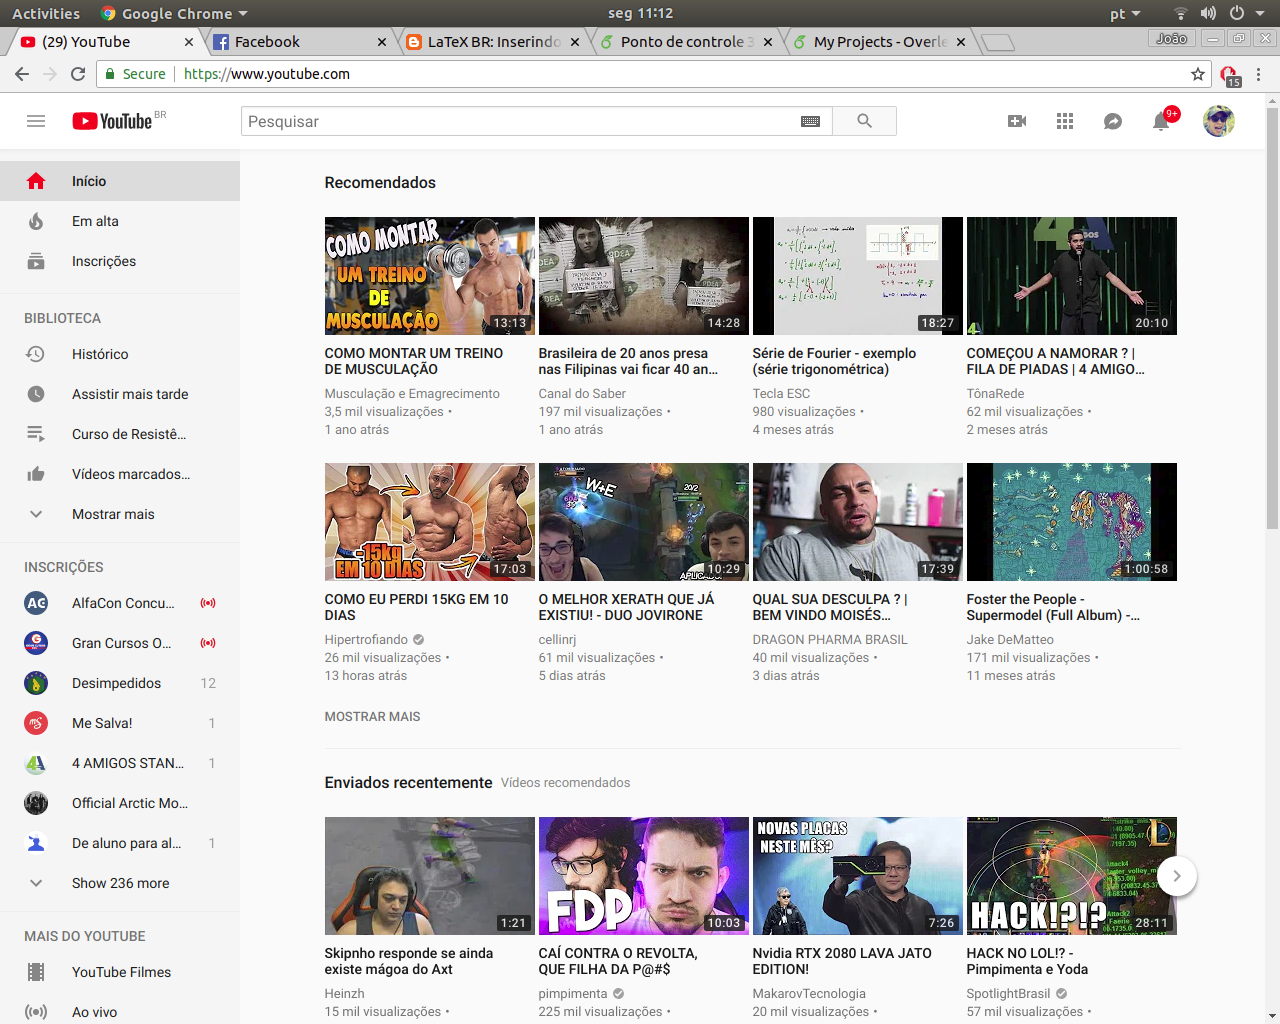
\includegraphics[scale=0.15]{nome_da_figura1.png}
		\caption{Figura 1}
		%\label{Rotulo}
\end{figure}

Os códigos e as figuras estão no GitHub, através do link:\href{https://github.com/helpthx}{https://github.com/helpthx}

%---------------------  ----------------------

\section{Resultado}
Os resultados foram conforme o esperado ao se juntar todos os componentes, entretanto houve algum problema na comunicação com o display 16x2, o qual não exibe as mensagens de trava e destrava do sistema de maneira correta, ou seja, em certos momentos caracteres estranhos são mostrados no display. Porem a comunicação entre o RC522, MSP430 e o rele esta totalmente funcional e a trava esta se comportando como deveria. Para os próximos passos será corrigido o problema do display e possivelmente adicionado mais funções ao sistema.

\begin{figure}[!ht]
		\centering
		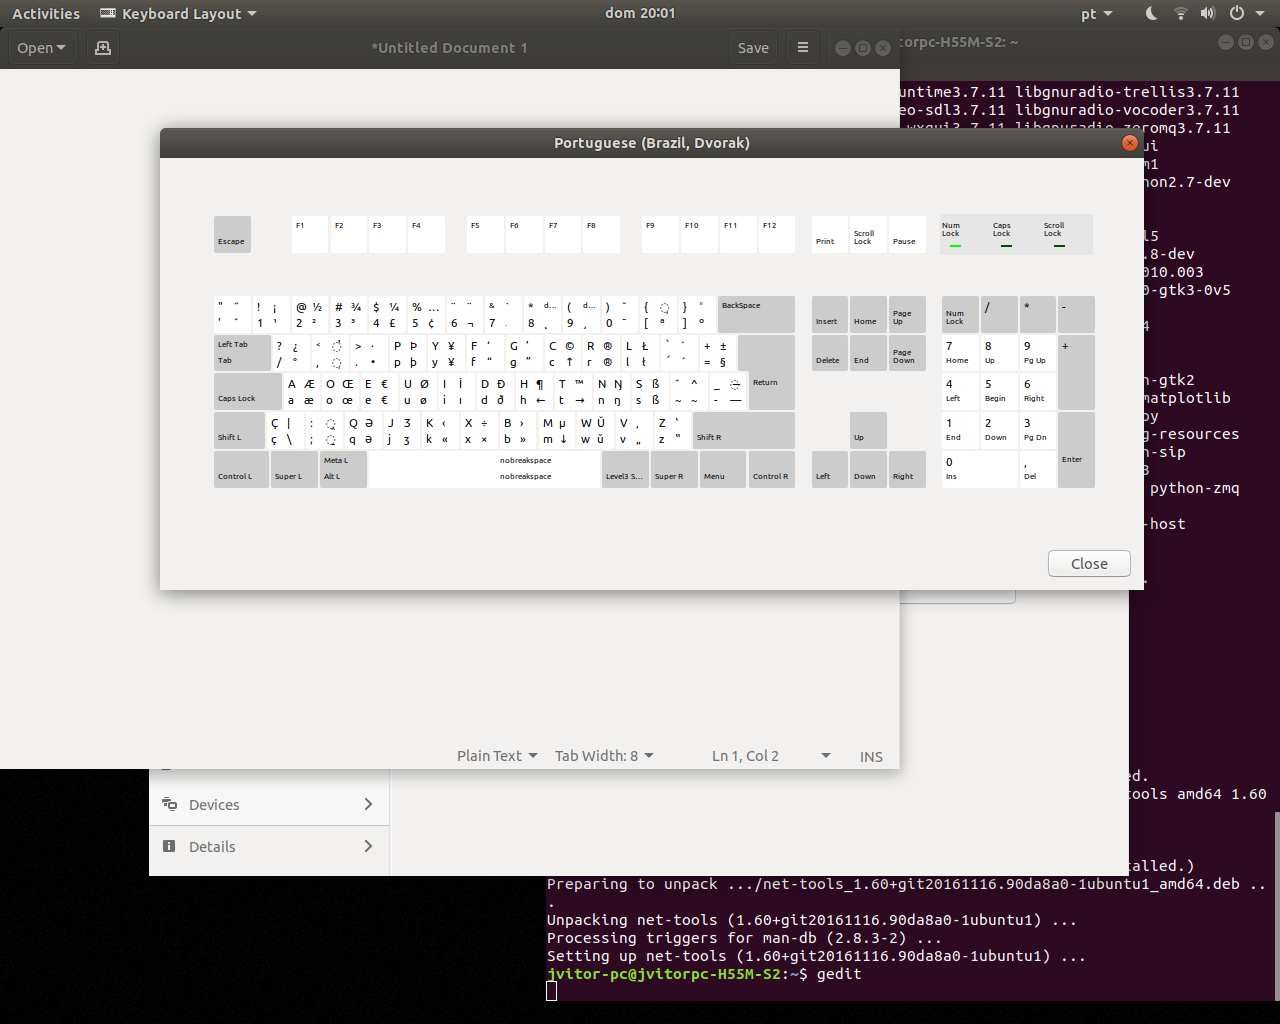
\includegraphics[scale=0.15]{nome_da_figura3.png}
		\caption{Figura 3}
		%\label{Rotulo}
\end{figure}

%---------------------  ----------------------

\section{Relação de Custo}
Até o presente momento se foi gasto em torno de R\$214,10 para o projeto, o que pode ser extremamente reduzido se as peças fossem compradas com certa antecipação, o MSP comprado direto pelo fornecedor a Texas, dessa maneira fazer com que o preço do projeto reduzido em mais de 50\% do valor atual, os outros componentes se comprando em grandes quantidades consegue-se uma grande redução de preços, o que viabilizaria a construção em maior escala do projeto com um menor preço e com certas melhorias uma possível entrada na concorrência de vendas de produtos pensados para segurança e controle de ambientes, como sendo uma alternativa de baixo custo que poderia ser modificada com necessidades do próprio cliente.



%-------------------- REFERÊNCIA -----------------
\begin{thebibliography}{1}


\bibitem{IEEEhowto:kopka}
H.~Kopka and P.~W. Daly, \emph{A Guide to \LaTeX}, 3rd~ed.\hskip 1em plus
  0.5em minus 0.4em\relax Harlow, England: Addison-
%FALTA ARRUMAR AS REFERÊNCIAS 

\end{thebibliography}




% that's all folks
\end{document}


